\documentclass[12pt]{article}

\usepackage{bbm}
\usepackage{fancyhdr}
\usepackage{titling}
\usepackage{enumitem}
\usepackage{amsmath}
\usepackage{dsfont}
\usepackage{amsfonts}
\usepackage{amssymb}
\usepackage{amsthm}
\usepackage{geometry}
\usepackage{tikz}
\usepackage{algorithm}
\usepackage{algpseudocode}
\geometry{verbose,tmargin=1in,bmargin=1in,lmargin=1in,rmargin=1in}
\renewcommand{\vec}[1]{\mathbf{#1}}
\newcommand{\dec}{\text{dec}}
\newcommand{\divi}{\mathbin{\textnormal{div}}}
\title{Homework 1}
\author{Satvik Prasad}
\date{}
\newtheorem{lemma}{Lemma}[section]
\fancypagestyle{plain}{%
  \fancyhf{}
  \fancyhead[L]{\theauthor}
  \fancyhead[R]{\thedate}
}
\pagestyle{plain}
\makeatletter
\def\@maketitle{%
  \newpage
  \null
  \vskip 1em%
  \begin{center}%
    \let \footnote \thanks
    {\LARGE \@title \par}%
    \vskip 1em%
  \end{center}%
  \par
\vskip 1em}
\makeatother
\usepackage{cmbright}

\newcommand{\mat}[1]{\mathbf{#1}}

% ---------- Probability theory ----------
% Core operators (optional argument-free; use as \E{X}, \Var{X}, \Cov{X}{Y})
\DeclareMathOperator{\EOp}{\mathbb{E}}
\DeclareMathOperator{\VarOp}{Var}
\DeclareMathOperator{\CovOp}{Cov}
\DeclareMathOperator{\CorrOp}{Corr}

\renewcommand{\P}[1]{\mathbb{P}\left(#1\right)}        % \P{A}
\newcommand{\E}[1]{\EOp\left[#1\right]}                % \E{X}
\newcommand{\Var}[1]{\VarOp\left(#1\right)}            % \Var{X}
\newcommand{\Cov}[2]{\CovOp\left(#1,\,#2\right)}       % \Cov{X}{Y}
\newcommand{\Corr}[2]{\CorrOp\left(#1,\,#2\right)}     % \Corr{X}{Y}
\newcommand{\SD}[1]{\operatorname{SD}\left(#1\right)}  % \SD{X}

% Subscripted versions, e.g. \Esub{\theta}{X}, \Psub{\theta}{A}
\newcommand{\Esub}[2]{\EOp_{#1}\left[#2\right]}
\newcommand{\Psub}[2]{\mathbb{P}_{#1}\left(#2\right)}

% Conditioning, indicators, independence
\newcommand{\given}{\,\middle|\,}                      % \E{X \given Y}
\newcommand{\ind}[1]{\mathbbm{1}\left\{#1\right\}}     % \ind{X > 0}
\newcommand{\indep}{\perp\!\!\!\perp}                  % X \indep Y
\newcommand{\iid}{\overset{\text{iid}}{\sim}}          % X_i \iid \Normal(0,1)

% Convergence
\newcommand{\convp}{\xrightarrow{\;p\;}}               % in probability
\newcommand{\convd}{\xrightarrow{\;d\;}}               % in distribution
\newcommand{\convas}{\xrightarrow{\text{a.s.}}}        % almost surely
\newcommand{\convLp}[1]{\xrightarrow{L^{#1}}}          % in L^p

% Probability spaces
\newcommand{\F}{\mathcal{F}}                           % sigma-algebra
\newcommand{\B}{\mathcal{B}}                           % Borel sigma-algebra
\newcommand{\pspace}{(\Omega, \F, \mathbb{P})}

% Common distributions
\newcommand{\Normal}{\mathcal{N}}
\newcommand{\Bern}{\operatorname{Bernoulli}}
\newcommand{\Bin}{\operatorname{Binomial}}
\newcommand{\Pois}{\operatorname{Poisson}}
\newcommand{\Unif}{\operatorname{Uniform}}
\newcommand{\Exp}{\operatorname{Exp}}
\newcommand{\Geom}{\operatorname{Geometric}}
\newcommand{\Gam}{\operatorname{Gamma}}
\newcommand{\Beta}{\operatorname{Beta}}

% Number sets
\newcommand{\R}{\mathbb{R}}
\newcommand{\N}{\mathbb{N}}
\newcommand{\Z}{\mathbb{Z}}


\begin{document}
\begin{enumerate}
    \item \textbf{Green Circle, 1} 
    To telescope, we write $4k = (k+1)^2 - (k -1)^2,$ yielding
    \begin{align*}
        \sum_{k = 1}^{n} k^3 &= \sum_{k = 1}^{n} k^2 \left(\dfrac{(k+1)^2 - (k-1)^2}{4}\right) \\
        &= \frac{1}{4}\left(\sum_{k = 1}^{n} k^2(k+1)^2 - \sum_{k = 1}^{n}k^2(k-1)^2\right) \\
        &= \frac{1}{4}\left(\sum_{k = 1}^{n} k^2(k+1)^2 - \sum_{k = 0}^{n - 1}(k + 1)^2k^2\right) \\
        &= \dfrac{1}{4}\left(n^2(n+1)^2\right) \\
        &= \left (\dfrac{n(n+1)}{2} \right)^2 \\
        &= \left( \sum_{k = 1}^{n} k \right)^2,
    \end{align*}
    using the well-known closed form of $1 + 2 + \ldots + n,$ and thus 
    \begin{align*}
        1^3 + 2^3 + 3^3 + \ldots  +n^3 = (1 + 2 + \ldots + n)^2
    \end{align*}
    as required.

    For a picture proof, we decompose a $1 + 2 + \ldots + n$ sided square tile into the following stripe pattern:

\begin{center}
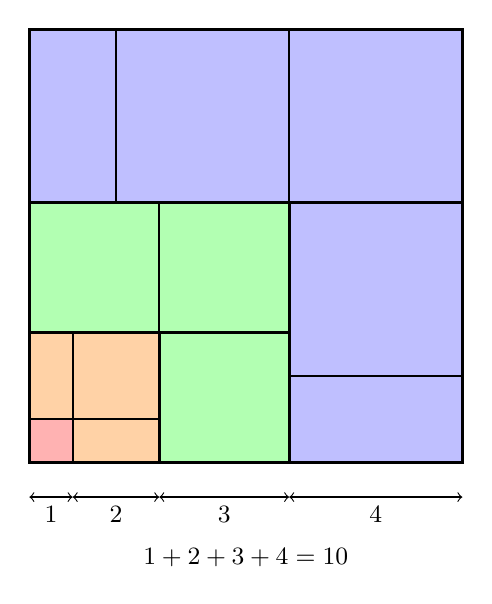
\begin{tikzpicture}[scale=0.55, every node/.style={font=\small}]

% ---- k = 1: one 1x1 square
\fill[red!30] (0,0) rectangle (1,1);

% ---- k = 2: gnomon [0,3]^2 \ [0,1]^2, two 2x2 squares (one split in halves)
\fill[orange!35] (1,1) rectangle (3,3);
\fill[orange!35] (1,0) rectangle (3,1);
\fill[orange!35] (0,1) rectangle (1,3);

% ---- k = 3: gnomon [0,6]^2 \ [0,3]^2, three 3x3 squares
\fill[green!30] (3,3) rectangle (6,6);
\fill[green!30] (3,0) rectangle (6,3);
\fill[green!30] (0,3) rectangle (3,6);

% ---- k = 4: gnomon [0,10]^2 \ [0,6]^2, four 4x4 squares (one split in halves)
\fill[blue!25] (6,6)  rectangle (10,10);
\fill[blue!25] (6,2)  rectangle (10,6);
\fill[blue!25] (6,0)  rectangle (10,2);
\fill[blue!25] (2,6)  rectangle (6,10);
\fill[blue!25] (0,6)  rectangle (2,10);

% ---- square outlines
\draw[thick] (0,0) rectangle (1,1);
\draw[thick] (1,1) rectangle (3,3);
\draw[thick] (3,3) rectangle (6,6)  (3,0) rectangle (6,3)  (0,3) rectangle (3,6);
\draw[thick] (6,6) rectangle (10,10) (6,2) rectangle (10,6) (2,6) rectangle (6,10);

% half-squares: outline, dashed line marking the cut
\draw[thick] (1,0) rectangle (3,1);   \draw[thick] (0,1) rectangle (1,3);
\draw[thick] (6,0) rectangle (10,2);  \draw[thick] (0,6) rectangle (2,10);
\draw[thick,dashed] (1,1) -- (3,1)  (1,1) -- (1,3);
\draw[thick,dashed] (6,2) -- (10,2) (2,6) -- (2,10);

% gnomon boundaries (nested squares of side T_k)
\draw[very thick] (0,0) rectangle (10,10);
\draw[very thick] (0,0) rectangle (6,6);
\draw[very thick] (0,0) rectangle (3,3);

% ---- side lengths
\draw[<->] (0,-0.8) -- (1,-0.8)  node[midway,below] {$1$};
\draw[<->] (1,-0.8) -- (3,-0.8)  node[midway,below] {$2$};
\draw[<->] (3,-0.8) -- (6,-0.8)  node[midway,below] {$3$};
\draw[<->] (6,-0.8) -- (10,-0.8) node[midway,below] {$4$};
\node at (5,-2.2) {$1+2+3+4 = 10$};

\end{tikzpicture}
\end{center}

The area of the $k$-th stripe is composed of $k$ tiles of side length $k,$ meaning the total area of $(1 + 2 + \ldots  + n)^2$ can be written as $\sum_{k = 1}^{n} k \cdot k^2 = \sum_{k = 1}^{n}k^3$ as required.

\item \textbf{Green Circle, 3} \begin{enumerate}
    \item We prove this inductively. For $n = 1,$ 
    \begin{align*}
        F_1 = 1 = 2 - 1 = F_3 - 1,
    \end{align*}
    meaning the statement is true for $n = 1.$

    Now, assume this is true for $1 \leq k \leq n,$  where $k, n$ are integers.

    Then, we have $$
    F_1 + F_2 + \ldots + F_{n+1} = F_{n + 2} - 1 + F_{n + 1} = F_{n + 3} - 1,
    $$
    meaning the statement is true for $n + 1,$ concluding our inductive step.

    Therefore, by strong induction, the statement is true.

    \item Base case: $F_1^2 = 1^2 = 1 \cdot 1 =  F_1 F_2.$

    Inductive step: Assume true for $1 \leq k \leq n,$ $n, k$ integers. Then, 
    \begin{align*}
        F_1^2 + F_2^2 + \ldots + F_{n+1}^2 &= F_n F_{n + 1} + F_{n + 1}^2 \\
        &= F_{n + 1}(F_n + F_{n + 1}) \\
        &= F_{n + 2} F_{n + 1},
    \end{align*}
    concluding our inductive step.

    Picture proof of the inductive step (can also fill in recursively till $F_0$):

\begin{center}
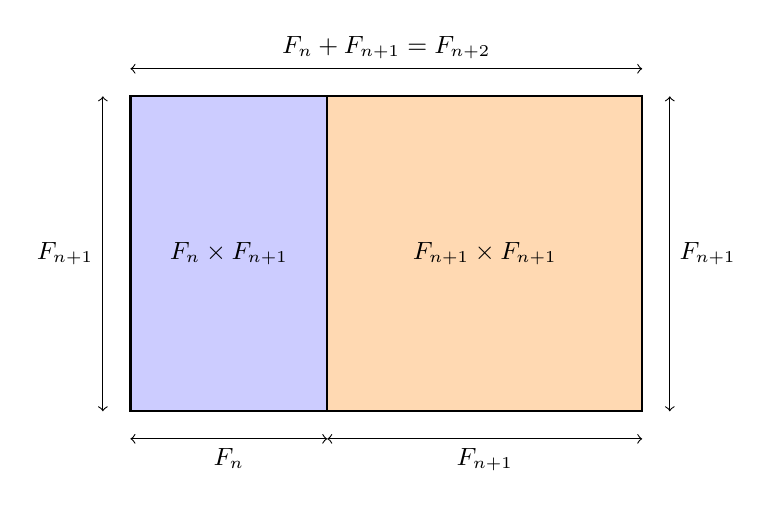
\begin{tikzpicture}[scale=0.5, every node/.style={font=\small}]

% drawing lengths (only used for proportions; change freely)
\def\a{5}   % stands for F_n
\def\b{8}   % stands for F_{n+1}

% F_n x F_{n+1} rectangle (inductive hypothesis)
\fill[blue!20] (0,0) rectangle (\a,\b);
\draw[thick]   (0,0) rectangle (\a,\b);
\node at ({\a/2},{\b/2}) {$F_n \times F_{n+1}$};

% F_{n+1} x F_{n+1} square attached along the side of length F_{n+1}
\fill[orange!30] (\a,0) rectangle ({\a+\b},\b);
\draw[thick]     (\a,0) rectangle ({\a+\b},\b);
\node at ({\a+\b/2},{\b/2}) {$F_{n+1} \times F_{n+1}$};

% side-length labels
\draw[<->] (0,-0.7)        -- (\a,-0.7)        node[midway,below] {$F_n$};
\draw[<->] (\a,-0.7)       -- ({\a+\b},-0.7)   node[midway,below] {$F_{n+1}$};
\draw[<->] (-0.7,0)        -- (-0.7,\b)        node[midway,left]  {$F_{n+1}$};
\draw[<->] ({\a+\b+0.7},0) -- ({\a+\b+0.7},\b) node[midway,right] {$F_{n+1}$};

% total width
\draw[<->] (0,{\b+0.7}) -- ({\a+\b},{\b+0.7})
      node[midway,above] {$F_n + F_{n+1} = F_{n+2}$};

\end{tikzpicture}
\end{center}
\end{enumerate}

\item \textbf{Green Circle, 4} Base case: $8 = 3 + 5,$ $9 = 3(3),$ $10 = 2(5).$

Inductive step: Assume true for all integers $k$ where $8 \leq k \leq n - 1$ for some integer $n > 10.$ Since $n > 10,$ $n - 3 \geq 8,$ meaning $n - 3$ lies within the range of the inductive hypothesis. 

Then, $$\underbrace{n - 3}_{8 \leq n -3 \leq n - 1} = 3a + 5b$$ for some non-negative integers $a, b,$ implying $n = 3(a + 1) + 5b.$ Thus, $a' = a + 1$ and $b' = b$ are non-negative integers such that $n = 3a' + 5b',$ concluding our inductive step.

Thus, every integer $n \geq 8$ can be written in such a form.

To find the largest integer that cannot be expressed as $4a + 7b$ for $a, b$ non-negative, notice that if we have a series of $4$ consecutive integers that can be expressed in this form, all subsequent integers can be expressed in this form via similar inductive reasoning. 

Let $k + 1, k + 2, \ldots k + 4$ denote the smallest $k$ for which $k + 1, \ldots, k + 4$ can be written in this form. Then, since $k$ is the smallest such integer, $k$ cannot be written in this form (otherwise $k, k +1, \ldots, k + 3$ would be a lesser contiguous streak). Every integer $n \geq k + 1$ can be expressed as $4a + 7b$ for non-negative integers $a, b,$ meaning $k$ must necessarily be the largest integer that cannot be written in that form.

In increasing order, integers that can be expressed in such a form are $$0, 4, 7, 11, 12, 14, 15, 16, \underbrace{18, 19, 20, 21}_{k +1 , \ldots k + 4}.$$ Hence, $17$ is the largest number that can't be expressed as $4a + 7b$ for non-negative integers $a, b.$

\item \textbf{Blue Square, 6} We proceed via induction. For $n = 1,$
$$
\dfrac{1}{2} \leq \dfrac{1}{\sqrt{3 + 1}},
$$
meaning it is true for $n = 1.$

Let us assume the statement is true for $n = k \geq 1,$ for integer $k.$ Then, 
\begin{align*}
\prod_{r = 1}^{k} \dfrac{2r - 1}{2r} \leq \dfrac{1}{\sqrt{3k + 1}},
\end{align*}
meaning $$
\prod_{r = 1}^{ k+ 1} \dfrac{2r - 1}{2r} \leq \dfrac{2k + 1}{(2k + 2)\sqrt{3k + 1}}.
$$

Assume for the sake of contradiction that
\begin{align*}
    \dfrac{2k + 1}{(2k + 2)\sqrt{3k + 1}} > \dfrac{1}{\sqrt{3k + 4}}.
\end{align*}
Then, this implies
\begin{align}
   \dfrac{(2k+1)^2}{(2k+2)^2}  > \dfrac{3k + 1}{3k + 4} \Rightarrow (2k + 1)^2(3k+4) > (3k+1)(2k+2)^2, \label{bsq6}
\end{align}
yielding 
$$
(4k^2 + 4k + 1)(3k + 4) > 4(k^2 + 2k + 1)(3k + 1),
$$
or equivalently, 
$$
12k^3 + 28k^2 + 19k + 4 > 12k^3 + 28k^2 + 20k + 4 \Rightarrow 19k > 20k,
$$
implying $19 > 20$ (since $k \geq 1$). This is a contradiction, and hence $$
    \dfrac{2k + 1}{(2k + 2)\sqrt{3k + 1}} \leq \dfrac{1}{\sqrt{3k + 4}},
$$
meaning 
$$
\prod_{r = 1}^{ k+ 1} \dfrac{2r - 1}{2r} \leq \dfrac{1}{\sqrt{3(k+1) + 1}},
$$
concluding our inductive step. $\therefore$ T by induction.

Trying \eqref{bsq6} with different coefficients, we get
$$
(2k + 1)^2(mk + 4) > 4(mk + 1)(k + 1)^2,
$$
which expands out to 
$$
4mk^3 + (4m + 16)k^2 + (m + 16)k + 4 > 4mk^3 + (8m + 4)k^2 + (4m + 8)k + 4,
$$
or equivalently, 
$$
(12 - 4m)k^2 + (8 - 3m)k > 0.
$$
Dividing by $k > 0,$ we get 
$$
(12 - 4m)k + 8 - 3m > 0,
$$
which is only vacuously false if \begin{align*}
12k  + 8 - (3 + 4k)m \leq 0 \Rightarrow m \geq \dfrac{12k + 8}{3 + 4k} &= \dfrac{(4k + 3) \cdot 3 - 1}{4k + 3} \\
&= 3- \dfrac{1}{4k + 3}
\end{align*}
for all $k > 0,$ requiring $m \geq 3$ to derive a contradiction during the inductive step.

\item We prove that every integer hvae such a representation, and that such a representation is unique. We prove this via induction. Base case: $N = 0$ has a unique representation given by $\epsilon_i = 0.$

Assume that all integers $0 \leq k \leq N - 1$ have a unique representation of that form, for some integer $N$. Let $n_0 = N \bmod 3.$ 

\begin{itemize}
\item If $n_0 = 2,$ then $0 \leq \dfrac{N + 1}{3} \leq N - 1$ since $N \geq 2,$ and thus $\dfrac{N + 1}{3} \in \mathbb Z$ is in the range of our inductive hypothesis. Thus, 
\begin{align*}
\dfrac{N + 1}{3} = \sum_{i \geq 0} \epsilon_i 3^{i} \Rightarrow N &= -1 + \sum_{i \geq 1}\epsilon_{i - 1} 3^{i}  \\
&= \sum_{i \geq 1} \delta_i 3^i,
\end{align*}
where $\delta_0 = -1,$ $\delta_k = \epsilon_{k - 1}$ for all $k > 0.$

\item Otherwise, if $n_0 \in \{0, 1\},$ $0 \leq \underbrace{\lfloor N/3}_{= (N - n_0)/3}\rfloor \leq N - 1,$ and thus we have 
\begin{align*}
   \dfrac{N - n_0}{3}  = \sum_{i \geq 0}\epsilon_i 3^i,
\end{align*}
meaning \begin{align*}
    N = n_0 + \sum_{i \geq 1}\epsilon_{i - 1}3^i = \sum_{i \geq 0} \delta _i 3^i,
\end{align*}
where $\delta_0 = n_0,$ $\delta_i = \epsilon_{i -1 }.$
\end{itemize}

In either case, we can write $N$ in the required form, meaning such a representation exists. Conversely, assume that such a representation is not unique.
\begin{itemize}
    \item For $n_0 = 2,$ this means we have two unique representations 
    $$
    \sum_{i \geq 0} \alpha_i 3^i, \qquad \sum_{i \geq 0} \beta_i 3^i,
    $$
    where at least one $\alpha_k \neq \beta_k.$ Since $N \equiv 2  \mod 3,$ $\alpha_0 = \beta_0 = -1.$ Then, 
    $$
    (N + 1)/3 = \sum_{i \geq 0} \alpha_{i + 1} 3^{i} = \sum_{i \geq 0} \beta_{i + 1}3^{i}.
    $$
    Since $(N + 1)/ 3$ must have a unique representation, $\alpha_{k} = \beta{k}$ for all $k \geq 1$ but $\alpha_0 = \beta_0.$ This contradicts our assumption, meaning $N$ has a unique representation.

    \item Similarly, for $n_0 \in \{0, 1\},$ we need $\alpha_0  = \beta_0 = n_0,$ meaning 
    \begin{align*}
        (N - n_0 )/ 3 = \sum_{i \geq 0} \alpha_{i+ 1} 3^{i} = \sum_{i \geq 0} \beta_{i + 1} 3^i.
    \end{align*}
    Using the same argument, this requires $\alpha_k = \beta_k$ for all $k \geq 1$ and $\alpha_0 = \beta_0 = n_0,$ meaning via contradiction $N$ must have a unique representation.
\end{itemize}

Thus, in all cases $N$ has a unique representation in the given form, concluding our inductive step.

$\therefore$ by strong induction, all integers $N \geq 0$ has a unique representation in such a form. For negative integers $N,$  $-N$ has a unique representation, and thus $N$ has representation given by $\epsilon_k^{'} = -\epsilon_k,$ where $\epsilon_k$ describes the rep. for $-N.$

\item \textbf{Black Diamond, 11} For our inductive step, notice that $$S_{n + 1} = S_n - \dfrac{1}{n + 1} + \dfrac{1}{2n + 1} + \dfrac{1}{2n + 2}.$$ Hence, we need some positive $f(n)$ such that 
$$
\frac{3}{4} - f(n) - \dfrac{1}{n + 1} + \dfrac{1}{2n + 1} + \dfrac{1}{2n + 2}  < \dfrac{3}{4} - f(n+ 1).
$$
Equivalently, we need 
\begin{align*}
f(n + 1) - f(n) < \dfrac{1}{n + 1} - \dfrac{1}{2n + 2} - \dfrac{1}{2n + 1}  &= \dfrac{1}{2n + 2} - \dfrac{1}{2n + 1}.
\end{align*}
To make things telescope, let's aim for a stricter requirement, namely
$$
f(n + 1) - f(n) \leq \dfrac{1}{2n + 2} - \dfrac{1}{2n} < \dfrac{1}{2n + 2} - \dfrac{1}{2n + 1} \Rightarrow f(n) - f(0) = \dfrac{1}{2n + 2},
$$
which is satisfied by 
$$
f(n) = \dfrac{1}{2n + 2}.
$$

For a base case, consider $S_3 = 1/4 + 1/5 + 1/6 = 37/60 < 5/8.$

Then, assume the statement is true for an integer $3 \leq n.$ Thus,
$$
S_n \sum_{i = n+1}^{2n} \dfrac{1}{i} < \dfrac{3}{4} - \dfrac{1}{2n + 2}.
$$
Therefore, we know
\begin{align*}
s_{n + 1} = \sum_{i = n + 2}^{2n + 2} \dfrac{1}{i} &< \dfrac{3}{4} - \dfrac{1}{2n + 2} + \dfrac{1}{2n + 2} + \dfrac{1}{2n + 1} - \dfrac{1}{n + 1} \\
&= \frac{3}{4} + \dfrac{1}{2n + 1} - \dfrac{1}{n + 1}.
\end{align*}

Assume for the sake of contradiction that 
$$
\dfrac{1}{x + 1} - \dfrac{1}{2x + 1} < \dfrac{1}{2x + 4}
$$
for integers $x \geq 3.$ Then, 
\begin{align*}
    \dfrac{x}{(x+1)(2x+1)} < \dfrac{1}{2x + 4} \Rightarrow 2x^2 + 4x < 2x^2 + 3x + 1,
\end{align*}
implying $$
x < 1,
$$
which is a contradiction. As a result, we know $$
\dfrac{1}{2n + 1} - \dfrac{1}{n + 1} \leq - \dfrac{1}{2n + 4}
$$ since $n \geq 3,$
meaning $$
S_{n + 1} < \frac{3}{4} - \dfrac{1}{2n + 4},
$$
concluding our inductive step.

$\therefore$ by induction, for $n \geq 3,$ $S_n < 3/4 - 1/(2n + 4) < 3/4.$ For $n = 1, 2$ $S_1 = 1/2 < 3/4$ and $S_2 = 7/12 < 9/12 = 3/4,$ meaning for all integers $n \geq 1,$
$$
    \dfrac{1}{n + 1} + \dfrac{1}{n + 2} + \ldots + \dfrac{1}{2n} < \dfrac{3}{4}.
$$

\item \textbf{Black Diamond, 12} \begin{enumerate}
    \item Consider an $n + 2$-gon. Consider any arbitrary partitioning $P$ of this into triangles formed by non-intersecting diagonals, and focus on a specific edge $e.$ 
    
    Edge $e$ must be including in the partitioning, and there are $n$ unique such triangles within the $n + 2$-gon formed by diagonals that have edge $e.$ Going clockwise, label $T_1$ the triangle with edge $e$ and vertex $v_1,$ $T_2$ the triangle with edge $e$ and vertex $v_2,$ all the way up to vertex $n.$

    Triangle $T_k$ splits the $n + 2$-gon into the triangle itself, a $k + 1$-gon (a $(k -1) + 2$-gon), and an $n + 2 - k$-gon (a $(n - k) + 2$-gon).

    Fixing $e$, every partitioning can be expressed as a selection on $T_k,$ and a partitioning on the induced polygons. Conversely, every selection on $T_k$ and a partitioning on the induced polygons selects a single partitioning of the $n + 2$-gon, meaning this is a bijection.

    Hence, the number of valid partitionings is 
    $$
    T_n = \sum_{k = 1}^{n} T_{k - 1} T_{n - k } = \sum_{k = 0}^{n - 1} T_{k} T_{n - k -1}.
    $$

    \item We proceed via induction. For $n = 0,$ $T_0 = 1 = \frac{1}{1} {0 \choose 0}.$

    Now, assume this is true for all integers $0 \leq k \leq n - 1,$ where $n \geq 1.$ Then, we have \begin{align*}
        T_n &= \sum_{k = 0}^{n-1}T_{k} T_{n - k - 1} \\
    \end{align*}
    This is the $n-1$-th coefficient of the polynomial described by
    $$
    \left(\sum_{k = 0}^{n-1} T_kx^k\right)^2 = \left( \sum_{k = 0}^{n-1} \dfrac{x^k}{k + 1} {2k \choose k} \right)^2.
    $$
    Hence, we need to find the $n - 1$-th coefficient of 
    $$
    f(x) = \left (\underbrace{\sum_{k \geq  0} {2k \choose k} \dfrac{x^k}{k + 1}}_{g(x)}\right)^2.
    $$

    Since $$
    (xg(x))' = \sum_{k \geq 0} {2k \choose k}x^k,
    $$
    consider the Maclaurin expansion for 
    $$
    (1+x)^{\alpha}
    $$
    for real $\alpha,$ yielding the series 
    $$
    \sum_{k \geq 0} \dfrac{\alpha(\alpha - 1) \ldots (\alpha -k + 1)}{k!} x^{\alpha - k}.
    $$
    Setting $\alpha = 1/2,$ we get
    \begin{align*}
(1 + x)^{-1/2}
&= \sum_{k \geq 0} \dfrac{(-1)(-3)(-5) \cdots (-(2k - 1))}{2^k \, k!} x^k \\
&= \sum_{k \geq 0} \dfrac{(-1)^{k} \, 1 \cdot 3 \cdots (2k - 1)}{2^k \, k!} x^k \\
&= \sum_{k \geq 0} \dfrac{(-1)^k \, (2k)!}{2^k \, k! \cdot 2^k \, k!} x^k \\
&= \sum_{k \geq 0} \dfrac{(-1)^k}{4^k} \binom{2k}{k} x^k    \end{align*}
    Setting $x = -4k,$ we get 
    $$
    \dfrac{1}{\sqrt{1-4x}} = \sum_{k \geq 0} {2k \choose k} x^k,
    $$
    meaning $(xg(x))' = \dfrac{1}{\sqrt{1 - 4x}}.$ Thus, 
    \begin{align*}
        xg(x) = -\frac{1}{2}\sqrt{1 - 4x} + C.
    \end{align*}
    At $x = 0,$ $-1/2 + C = 0,$ meaning we have 
    \begin{align*}
        g(x) = \frac{1}{2x}(1 - \sqrt{1 - 4x})
    \end{align*}
    on $x \neq 0, |x| \leq 1,$ i.e., 
    \begin{align*}
        f(x) &= \dfrac{1}{2x^2} \left( 
            1 - 2x -  \sqrt{1-4x} 
        \right) \\
        &= \frac{1}{2x^2} (2xg(x) - 2x) = \dfrac{g(x) - 1}{x} \\
        &= x^{-1}\left (\sum_{k \geq 0} {2k \choose k}\dfrac{x^k}{k + 1} -1\right) \\
        &= \sum_{k \geq 0} {2(k + 1) \choose k + 1} \dfrac{x^{k + 1}}{k+2},
    \end{align*}
    whose $n - 1$-th coefficient is $$\dfrac{{2n \choose n}}{n + 1}.$$ Therefore, $T_n = {2n \choose n }/(n+1),$ concluding our inductive step.

    \item Since $T_n$ is an integer, ${2n \choose n} = T_n(n + 1),$ where $T_n$ is an integer, meaning $n + 1 \mid {2n \choose n}.$
\end{enumerate}

\item \textbf{Black Diamond, 13} We have a sequence of $n$ integers $x_1, \ldots x_n$ whose sum is $1.$ Let $S_k$ be the rightmost least partial sum of the unshifted sequence, given by 
\begin{align*}
    S_k = \sum_{i =1}^{k} x_i.
\end{align*}
Then, we know \begin{align*}
    \sum_{i = k + 1}^{n} x_i = 1 - S_k.
\end{align*}

Then consider the sequence $$\{x_{k + 1}, x_{k + 2}, \ldots, x_{n}, x_1, \ldots, x_k\}.$$
Let the partial sums of this sequence be denoted by $S'.$ If an arbitrary $i$-the of the first $n - k$ partial sums are non-positive, then $S_{k + i} = S_k + S'_i \leq S_k,$ contradicting the minimality of $S_k,$ since $k$ is the largest such minimal index.

Additionally, if $S_j' \leq  0$ for $j > n - k,$ then \begin{align*}
    1 - S_k + S_{j - (n - k)} \leq  0,
\end{align*}
meaning \begin{align*}
    S_{j - (n-k)} \leq S_k - 1,
\end{align*}
which also contradicts the minimality of $S_k.$

Hence, none of the partial sums of this modified sequence is negative, meaning there exists a cyclic shift of such a sequence with all partial sums non-negative.

\item \textbf{Black Diamond, 14} We prove existence via induction, fixing $m.$ For $n = 1,$ a sequence of length $m + 1$ has two cases:
\begin{itemize}
    \item There is an increasing subsequence of length $2,$ in which the statement is trivially true,
    \item Otherwise, $x_{k + 1} < x_k$ for all valid indices $k,$ meaning the sequence is strictly decreasing and the sequence itself is a decreasing subsequence of length $m + 1.$ 
\end{itemize}
Hence, the statement is true for $n = 1.$

Assume T for all $1 \leq n \leq k - 1.$ Consider the subsequence $\mathcal K'$ of length
$$
mk + 1,
$$
where we are appending on $m$ distinct real numbers. If there is a decreasing subsequence of length $k + 1,$ then the statement is T for $n = k.$

Hence, assume we don't have a decreasing subsequence of length $k + 1.$ We must inductively show that in this case there is some increasing subsequence of length $m + 1$ instead.

Consider all subsequences of length $k$ in $\mathcal K'.$ Denote $\mathcal S_0$ the first (leftmost starting) of these subsequences, $\mathcal S_1$ the next leftmost, etc. Denote $N$ to be the number of such subsequences. We have two cases:
\begin{itemize}
    \item If $N < m + 1,$ remove the first element of all $\mathcal S_i$ from $\mathcal K'.$ This leaves a sequence of length $\geq m(k -1) + 1,$ and we can apply our inductive hypothesis to an arbitrary length $m(k-1) + 1$ subsequence. Call such a sequence $\mathcal K.$ Notice that $\mathcal K$ cannot contain a decreasing subsequence of length $k,$ since we removed the first element of all such subsequences from $\mathcal K',$ and $\mathcal K'$ contained no longer subsequences.
    
    Thus, by our inductive hypothesis $\mathcal K$ must contain an increasing subsequence of length $m + 1,$ meaning $\mathcal K'$ does too.

    \item Otherwise, $N \geq m + 1.$ In this case, consider the first element of all such $\mathcal S_i,$ denoted $a_i.$ If $a_i > a_j$ for some $j > i,$ then we can construct a decreasing subsequence of length $k + 1,$ which is a contradiction. Thus, $\{a_i\}$ is an increasing subsequence of length $\geq m + 1,$ meaning we can find an increasing subsequence of length $m + 1$ in $\mathcal K'$
\end{itemize}

In all cases, we can construct either an increasing subsequence of length $m + 1$ in $\mathcal K',$ or a decreasing subsequence of length $k + 1,$ concluding our inductive hypothesis.

$\therefore$ by induction, a sequence of distinct real numbers of length $mn + 1$ contains either an increasing subsequence of length $m$ or a decreasing subsequence of length $n + 1.$

Now, we prove that this is the smallest such length by constructing a sequence of length $mn$ that violates the constraints, i.e., must contain neither an increasing subsequence of length $m + 1,$ or a decreasing subsequence of length $n + 1.$ 

WLOG, assume $m \leq n.$ Define 
$N_i = \{i + 1, i + 2, \ldots, i + m\},$
and consider the sequence constructed as
$$
\mathcal S = \{N_n; N_{m -1}; \ldots; N_{1}\}.
$$
Since for $j > i,$ all the elements in $N_{j}$ are less than the elements in $N_{i},$ the longest increasing subsequence is length $m.$ Additionally, since $N_k$ is increasing for any $k,$ any decreasing subsequence must have at most one element in each $N_k,$ meaning $n$ is the upper bound on the length of a decreasing subsequence. Hence, we've constructed $\mathcal S$ such that it has no increasing subsequence of length $m + 1,$ and no decreasing subsequence of length $n + 1.$

If otherwise, we had $m \geq n,$ we could similarly construct decreasing $M_i,$ and append those together for a similar argument.

Thus, length $mn + 1$ is the smallest length to guarantee that a sequence composed of unique real numbers contains an increasing subsequence of length $m + 1$, or a decreasing subsequence of length $n + 1.$

\item \begin{enumerate}
    \item \textbf{Note: should specify positive $a_1, \ldots, a_n$.}
    For our base case, $a_1 \geq 1.$ Now, assume this statement is true for an integer $n \geq 1.$ Then, consider $a_1, \ldots, a_{n + 1}$ with product $1.$

    Apply the hypothesis to the $n$ elements 
    $$
    \{\sqrt[n]{a_k} \cdot a_i : i \neq k\},
    $$
    where $a_k > 0,$ yielding 
    \begin{align*}
    \sqrt[n]{a_k} \left(
    S - a_k
    \right) \geq n,
    \end{align*}
    meaning \begin{align*}
    S \geq \dfrac{n}{\sqrt[n]{a_k}} + a_k.
    \end{align*}

    Consider the function $f: \mathbb R^{+} \to \mathbb R$ defined as $$f(t)  = \dfrac{n}{t} + t^n .$$

    Differentiating, we get \begin{align*}
        f'(t) = \dfrac{nt^{n + 1} - n}{t^2},
    \end{align*}
    which is minimized when $t = 1.$ Since $f''(t) = n(n-1)t^{n-2} + 2nt^{-2},$ we have $f''(1) = n(n-1) + 2n = n^2 + n \geq 2,$ meaning this is a local minimum. Therefore, $S \geq f(1) = n + 1$ as required for our inductive step.

    \item For arbitrary $a_1, \ldots, a_n,$ let $b_i = \dfrac{a_i}{\sqrt[n]{a_1 a_2 \cdot a_n}},$ and thus the product of $b_1, \ldots, b_n$ is 1. As a result, we can deduce \begin{align*}
        \dfrac{a_1}{\sqrt[n]{a_1 a_2 \ldots a_n}} + \dfrac{a_2}{\sqrt[n]{a_1 a_2 \ldots a_n}} + \ldots + \dfrac{a_n}{\sqrt[n]{a_1 a_2 \ldots a_n}} \geq n,
    \end{align*}
    meaning \begin{align*}
        \dfrac{a_1 + \ldots + a_n}{n} \geq \sqrt[n]{a_1 a_2 \ldots a_n}
    \end{align*}
    as required.

    \item The Cauchy route is fairly intuitive, since it makes sense that proving $n \to 2n$ is tractable, and proving $n \to n - 1$ requires a substitution for $x_n$ in terms of the other elements, but requires a different form of induction (forward-backward).

    This route requires a large jump to proving the subset of cases where their product is $1$ (essentially a change of variables), but the induction becomes more straightforward.
\end{enumerate}
\end{enumerate}
\end{document}